\documentclass[conf]{new-aiaa}
%\documentclass[journal]{new-aiaa} for journal papers
\usepackage[utf8]{inputenc}

\usepackage{tgbonum}
\usepackage{graphicx}
\usepackage{caption}
\usepackage{subcaption}
\usepackage{amsmath}
\usepackage[version=4]{mhchem}
\usepackage{siunitx}
\usepackage{longtable,tabularx}
\setlength\LTleft{0pt} 
\usepackage{xcolor, soul}
\sethlcolor{green}
\usepackage{float}
\usepackage{mathabx}
\usepackage{rotating}
\usepackage{tikz}
\usepackage{setspace}
\usepackage{listings}
\lstdefinestyle{myListingStyle} 
    {
        basicstyle = \small\ttfamily,
        breaklines = true,
    }
\doublespacing

%% Preamble stuff
%Preamble
\usepackage{xcolor, soul}
\sethlcolor{yellow}



\title{Decision Making Under Uncertainty: Homework 1}

\author{Julian Lema Bulliard\footnote{Graduate Student, Aerospace Engineering Department}}
\affil{University of Colorado Boulder}

\begin{document}

\maketitle

\section{Questions}

\subsection{Question 1}
\begin{enumerate}[label = \alph*)]
    \item When we look at the table, we notice that the addition of all the outcomes does not equal 1.00, but instead adds up to 0.89\%. The final combination that is missing in the table is $A = 0$, $B = 0$, and $C = 0$. Therefore...
        \hl{P($A = 0$, $B = 0$, $C = 0$) = 11\%}


    \item For the marginal distribution of $A$ we can create the following table...\\
        \begin{tabular}{cc|cc}
            A & B & A=0 & A=1\\
            \hline
            0 & 0 & 0.14 & 0.11\\
            0 & 1 & 0.18 & 0.15\\
            1 & 0 & 0.29 & 0.05\\
            1 & 1 & 0.07 & 0.01\\
            \hline
             & & 0.68 & 0.32\\
        \end{tabular}
        
        Therefore, the marginal distribution of A is as follows: \hl{P($A = 0$) = 68\% and P($A = 1$) = 32\%}

    \item For the conditional distribution of $A$, we need to find $P(A=0|B=0,C=1)$ and $P(A=1|B=0,C=1)$

    This can be done by utilizing the following equations:

    \[P(A=0|B=0,C=1) = \frac{P(A = 0 , B = 0 , C = 1)}{P(B = 0 , C = 1)} = \frac{0.15}{0.15 + 0.18} = 0.4545\]\\
    \[P(A=1|B=0,C=1) = \frac{P(A = 1 , B = 0 , C = 1)}{P(B = 0 , C = 1)} = \frac{0.18}{0.15 + 0.18} = 0.5454\]

    To make sure we are getting sensible numbers, we always add up our results to ensure that they equal one. In this case, they do! \\
\end{enumerate}
\pagebreak

\subsection{Question 2}

For this question, let's first write out all the given information:

\begin{itemize}
    \item In women who participate in a screening
    \begin{itemize}
        \item 2\% have breast cancer - $P(C = 1) = 0.02$
        \item 98\% do not have breast cancer - $P(C = 0) = 0.98$
    \end{itemize}

    \item In women who have breast cancer (2\%)
    \begin{itemize}
        \item Positive Mammogram = 86\% (Truthful) - $P(M = 1|C = 1) = 0.86$
        \item Negative Mammogram = 14\% (False Negative) - $P(M = 0|C = 1) = 0.14$
    \end{itemize}

    \item In women who do not have breast cancer (98\%)
    \begin{itemize}
        \item Positive Mammogram = 8\% (False Positive) - $P(M = 1|C = 0) = 0.08$
        \item Negative Mammogram = 92\% (Truthful) - $P(M = 0|C = 0) = 0.92$
    \end{itemize}
\end{itemize}

For this question, we are tasked with finding the probability that if a woman had a positive mammogram, she actually has cancer. We could write this as
$P(C = 1|M = 1)$, where $C$ is one if she has cancer, and $M$ is one if she had a positive mammogram. 

Since we are given the information in 'reverse' we will need to apply Bayes' Rule to find the 'reverse' probability. 

\[P(C = 1)|M = 1) = \frac{P(M = 1|C = 1) \cdot P(C = 1)}{P(M = 1)}\]

We need to find $P(M = 1)$, we can use the marginal relationship equation of: \[P(M = 1) = P(M = 1|C = 1)\cdot P(C=1) + P(M = 1|C = 0)\cdot P(C=0) = 0.86 * 0.02 + 0.08 * 0.98 = 0.0956\]
Now we can continue

\[P(C = 1)|M = 1) = \frac{P(M = 1|C = 1) \cdot P(C = 1)}{P(M = 1)} = \frac{0.86 * 0.02}{0.0956} = 0.1799 = 17.99\%\]

\begin{center}
    \hl{$P(C = 1)|M = 1) = 17.99$}
\end{center}

\subsection{Question 3}
\begin{enumerate}[label = \alph*)]
\item 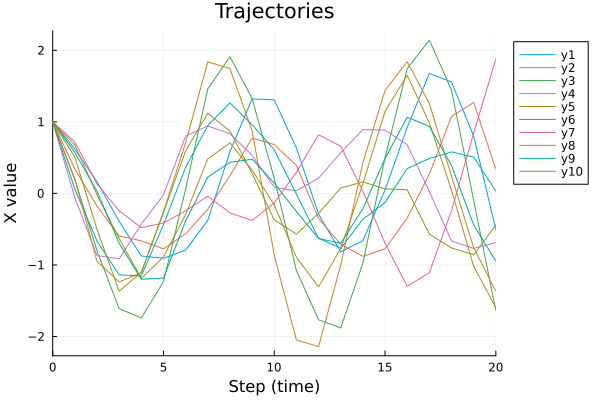
\includegraphics[scale = 0.60]{HW3Num3.png}
\item This is not a Markov Process since this process depends on $x_{t-1}$ and $x_t$
\item From the graph itself, it is hard to convince yourself that the process is Markov. If we truly did have a Markov process, our graph over time would resemble a 'random-walk' graph in which there would (shouldn't) be a pattern over time. Our graph clearly does not resemble this as ours has an oscillatory tendency over time. From class, we could also try to see if $P(s_{t+1}|s_t) = P(s_{t+1}|s_t , s_{t-1} , ..., s_0)$ how this would be calculated is another question, and whether it could be done is another. Overall, we can argue that it is not Markov due to its tendency of following a pattern
\item To create a Markov process, our state could only consist of the current state and the previous state, of course, including any other states would null the Markov process. To do this we would define...

\begin{gather}
    y_t
    =
    \begin{bmatrix}
        x_{t-1}\\
        x_{t}
    \end{bmatrix}
\end{gather}


\begin{gather}
    y_{t+1}
    =
    \begin{bmatrix}
        0 & 1\\
        -1 & 1.5
    \end{bmatrix}
    y_t + 
    \begin{bmatrix}
        0\\
        1
    \end{bmatrix}
    v_t
\end{gather}

When going through the matrix math we obtain

\[x_t = x_t\] Which we would hope is correct
\[x_{t+1} = 1.5 x_t - 1 x_{t-1} + v_t\] This is our original equation that only includes the previous state. 

\end{enumerate}

\subsection{Question 4}

The results for this section are seen in the auto-generated .json file below. 

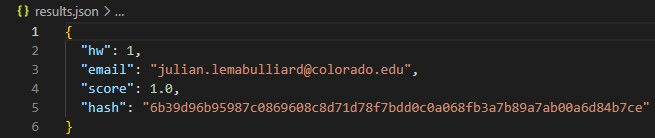
\includegraphics[]{json.jpg}

\section{Code Appendix}
\begin{verbatim}
    import DMUStudent.HW1

using Random
using Distributions
using Plots
#-------------
# Testing
#-------------

# x = randn(10,10)
# y = 1:10
# plot(y , x[1,:])

#------------- 
# Problem 3
#-------------
# See https://github.com/zsunberg/CU-DMU-Materials/blob/master/notebooks/030-Stochastic-Processes.ipynb for code that simulates a stochastic process.

# First let's create a function outputs the step
function step(xt , x_tm1)
    mu = 0
    sigma2 = 0.04
    sigma = sqrt(sigma2)
    # vt = randn() * sigma + mu
    x_tp1 = 1.5*xt - x_tm1 + rand(Normal(mu,sigma))

    return x_tp1
end

# Function to be called to create history
function simulate(step; n_steps = 20 , xt = 1.0, xtm1 = 1.0)
    # Pre allocate the first two given variables
    history = [xtm1 , xt]

    for _ in 1:n_steps
        
        # Store the first variables as above to xtm1 and xt
        # Step to the next number and store this to history
        # On next step these new numbers will be interchanged with xt and xtm1

        xtm1 , xt = history[end-1:end]
        xtp1 = step(xt,xtm1)
        push!(history,xtp1)

    end
    # Return history 
    return history
end


# Iterate ten, twenty step trajectories
sims = 10
steps = 20
store = zeros(22,sims)
for i in 1:sims
    store[:,i] = simulate(step)
end
storeplot = store[2:end,:];

row , col = size(store)
output = plot(0:row-2, storeplot , legend =:outertopright)
title!(output, "Trajectories")
xlabel!(output, "Step (time)")
xlims!(output,0,20)
ylabel!(output, "X value")
png(output,"HW3Num3")




#------------- 
# Problem 4
#-------------

function f(a , bs)
    # Finding the size of the matrix and initializing a new matrix
    result = a*bs[1]

    for i in 2:length(bs)
        result = max.(result , a*bs[i])
    end
    
    @show typeof(result)
    return result
end

# # This is how you create the json file to submit
HW1.evaluate(f, "julian.lemabulliard@colorado.edu")
\end{verbatim}
\end{document}